\section{Discussion}

In physics, the Navier–Stokes equations, named after Claude-Louis Navier and George Gabriel Stokes, describe the motion of viscous fluid substances.

\autoref{eq:Incompressible Navier-Stokes} shows the incompressible Navier-Stokes equations using tensor notation.

\begin{equation}
    \frac{\partial u_i}{\partial t} + u_j \frac{\partial u_i}{\partial x_j} = -\frac{1}{\rho} \frac{\partial P}{\partial x_i} + \nu \frac{\partial^2 u_i}{\partial x_j^2}
    \label{eq:Incompressible Navier-Stokes}
\end{equation}

\begin{figure}[H]
    \centering
    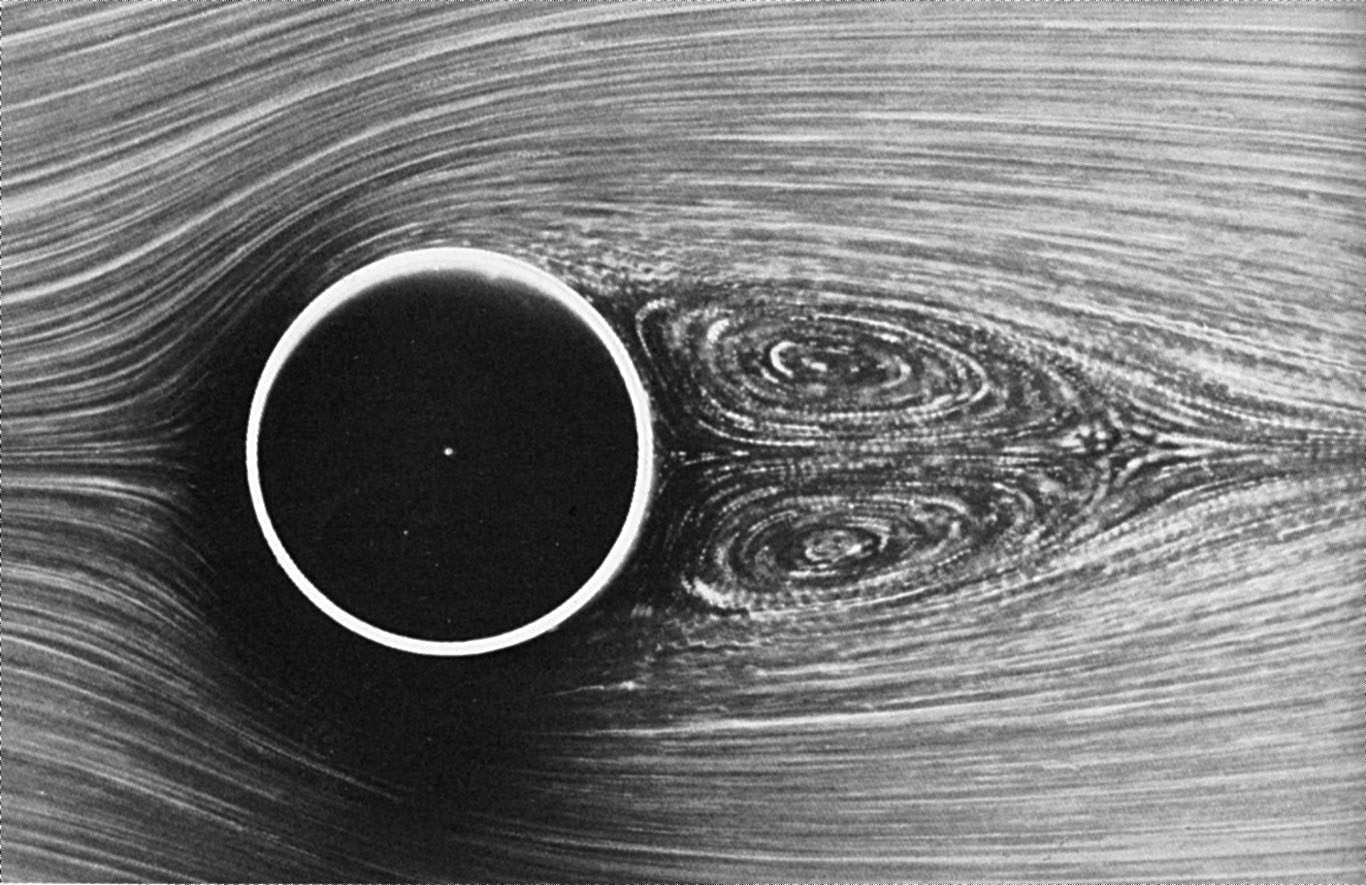
\includegraphics[width=0.5\textwidth]{Images/CylinderImage.jpg}
    \caption[Caption used in list of tables]{Caption written below figure.}
    \label{fig:flow around cylinder}
    \source{Insert image source here}
\end{figure}

